\documentclass[border=10pt]{standalone}
\usepackage{tikz}
\usetikzlibrary{positioning,fit,arrows.meta,calc}

\begin{document}
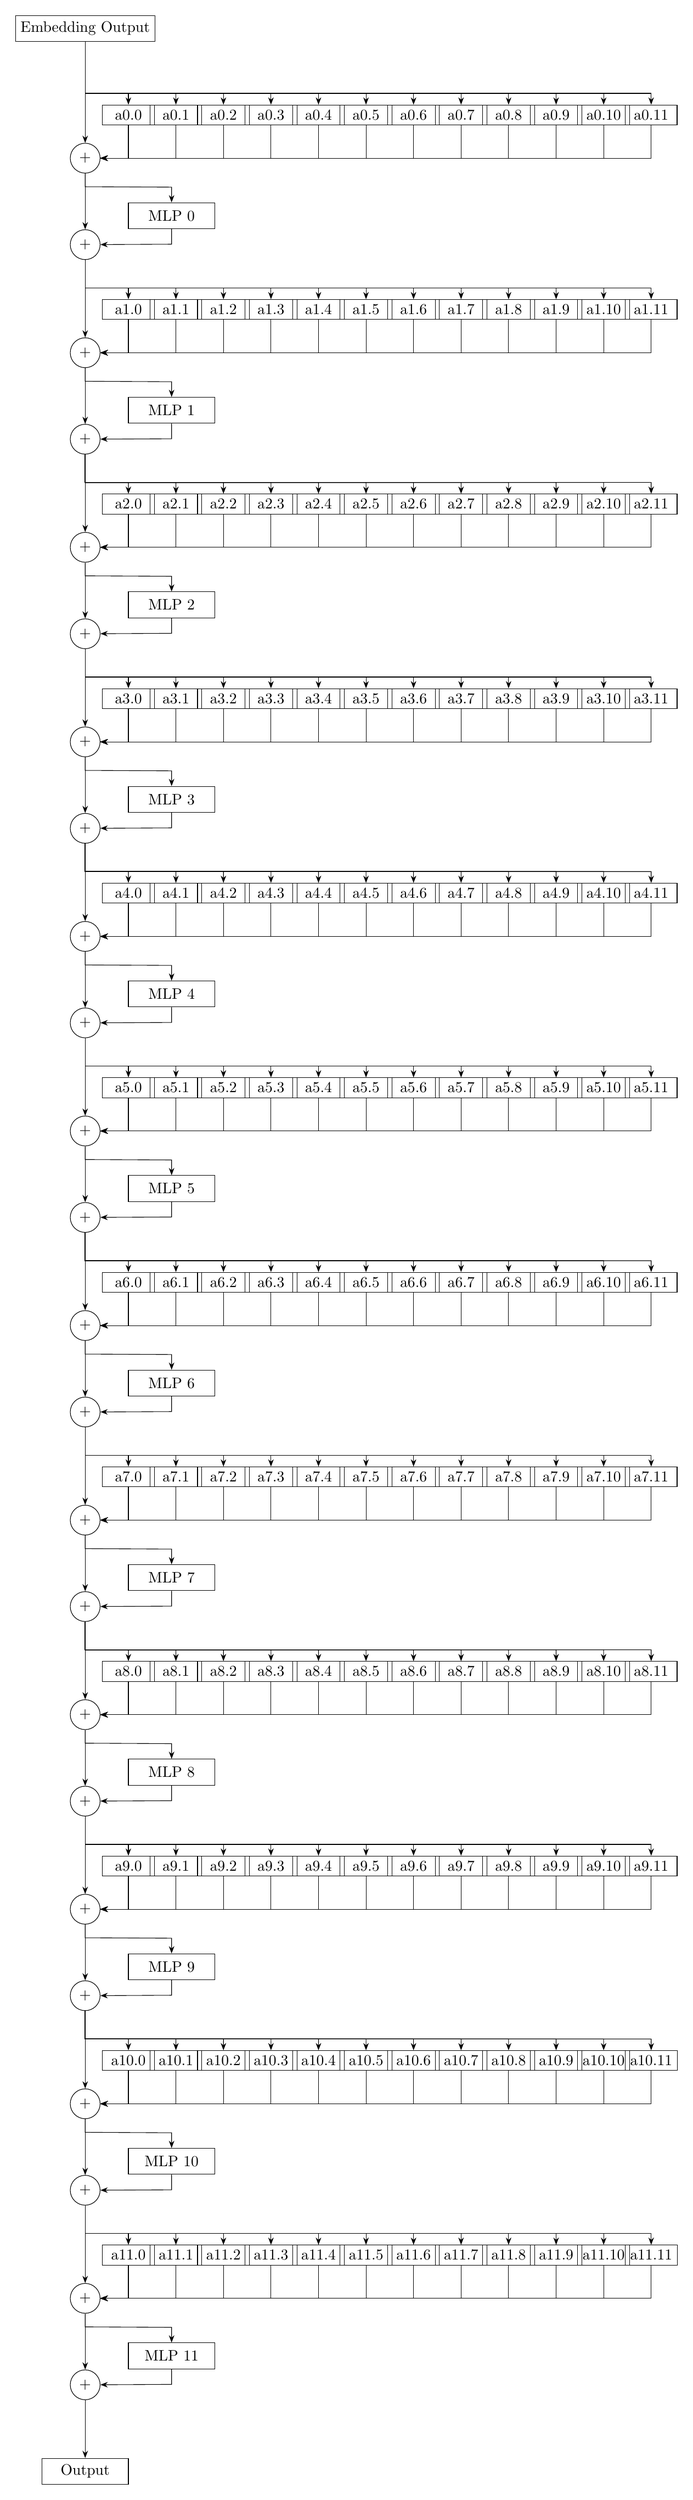
\begin{tikzpicture}[
    box/.style={rectangle,draw,minimum width=2cm,minimum height=0.6cm},
    attention/.style={rectangle,draw,minimum width=1.2cm,minimum height=0.4cm},
    layer/.style={rectangle,draw,dashed,inner sep=0.3cm},
    arrow/.style={-Stealth}
]

\def \LAYERHEIGHT {4.5}; % height of a layer

% Input
\node[box] (input) at (0,0) {Embedding Output};

% Define a style for attention head column
\foreach \l in {0,...,11} {
    % Layer label and box
    % \node[layer,below=0.8cm of input.south] (layer\l) {};
    % \node[left] at (layer\l.west) {Layer \l};
    \pgfmathsetmacro \lPrevious {int(\l - 1)}
    % Attention heads
    \foreach \h in {0,...,11} {
        \node[attention] (a\l\h) at ($(1+\h*1.1,-2-\l*\LAYERHEIGHT)$) {a\l.\h};
        \ifnum \l > 0
            \draw[arrow] (concat_mlp\lPrevious) -- ($(concat_mlp\lPrevious)-(0,1.0)$) -- ($(a\l\h)+(0,0.5)$) -- (a\l\h);
        \fi
    }

    % Connect previous layer's MLP to current layer attention heads
    
    
    % Concatenation for attention heads at each layer
    \node[circle,draw] (concat_att\l) at (0,-3-\l*\LAYERHEIGHT) {+};
    
    % Connect attention heads to concat
    \foreach \h in {0,...,11} {
        \draw[arrow] (a\l\h) -- ($(a\l\h)-(0,1)$) -- (concat_att\l);
    }

    % MLP for each layer
    \node[box] (mlp\l) at (2,-4.33-\l*\LAYERHEIGHT) {MLP \l};
    
    % Connect concatenation for attention heads to MLP (and to MLP concatenation of previous layer if current layer > 0)
    \draw[arrow] (concat_att\l) -- ($(concat_att\l)-(0,0.66)$) -- ($(mlp\l)+(0,0.66)$) -- (mlp\l);
    \ifnum \l > 0
        \draw[arrow] (concat_mlp\lPrevious) -- (concat_att\l);
    \fi

    % Concatenation for MLP at each layer
    \node[circle,draw] (concat_mlp\l) at (0,-5-\l*\LAYERHEIGHT) {+};

    % Connect concatenation for attention heads to concatenation for mlp and mlp itself
    \draw[arrow] (concat_att\l) -- (concat_mlp\l);
    \draw[arrow] (mlp\l) -- ($(mlp\l)-(0,0.66)$) -- (concat_mlp\l);
    
    
    
    % % Connect to next layer or output
    % \ifnum\l<12
    %     \draw[arrow] (mlp\l) -- ($(mlp\l)+(0,-0.3)$); -> IS HOW YOU CAN CALL THE COORDINATES OF AN ALREADY DRAWN NODE (basically math inside the tikz env.
    % \fi
}

% Connect input to first layer attention heads and its concatenation
\foreach \h in {0,...,11} {
    \draw[arrow] (input) -- ($(input)-(0,1.5)$) -- ($(input)+(1+\h*1.1,-1.5)$) -- (a0\h);
}
\draw[arrow] (input) -- (concat_att0);

% Output
\node[box] (output) at (0,-7-11*\LAYERHEIGHT) {Output};
\draw[arrow] (concat_mlp11) -- (output);

\end{tikzpicture}
\end{document}